\documentclass[a4paper,conference]{IEEEtran}
\IEEEoverridecommandlockouts

\usepackage{cite}
\usepackage{amsmath,amssymb,amsfonts}
\usepackage{graphicx}
\usepackage{textcomp}
\usepackage{xcolor}
\usepackage{booktabs}
\usepackage{multirow}
\usepackage{array}
\usepackage{tikz}
\usetikzlibrary{arrows.meta, positioning, shapes.geometric}
\usepackage[hidelinks]{hyperref}
\usepackage{subcaption}

\def\BibTeX{{\rm B\kern-.05em{\sc i\kern-.025em b}\kern-.08em
    T\kern-.1667em\lower.7ex\hbox{E}\kern-.125emX}}

\begin{document}

\title{Anatomy-Aware Routing for Robust Medical Image Segmentation: A Failure-Detectable Alternative to Mixed Models}

\author{\IEEEauthorblockN{Musab Ahmed Khan}
\IEEEauthorblockA{\textit{Sabanci University}\\musabahmedkhan22@gmail.com}
\and
\IEEEauthorblockN{Mohammed Sateh Salem}
\IEEEauthorblockA{\textit{Sabanci University}\\satehsalam52@gmail.com}}

\maketitle

\IEEEpubid{\makebox[\columnwidth]{\textbf{979-8-3195-1046-4/26/\$31.00 \copyright{}2026 IEEE}\hfill}%
\hspace{\columnsep}\makebox[\columnwidth]{}}

\begin{abstract}
Heterogeneous medical segmentation pipelines that use a single shared model lose organ-specific feature learning and degrade silently under distribution shift. We propose an anatomy-aware framework where an upstream classifier routes inputs to dedicated specialist networks, combined with a composite post-hoc failure detector based on MC-Dropout uncertainty, domain-shift detection, and plausibility checking. Using chest X-ray pneumothorax and brain MRI datasets, we show anatomy-aware routing yields higher segmentation accuracy (+8.6--14.4 Dice points) compared to a mixed-organ baseline. Our failure detector achieves flag rates of 1.000 on misrouted pneumothorax cases and 0.963 on brain cases. In contrast, under identical noise, the mixed model produces flag rates of only 0.173 and 0.156. Anatomy-aware pipelines offer superior accuracy and the ability to \emph{fail loudly}, allowing safer clinical deployment through explicit abstention.
\end{abstract}

\begin{IEEEkeywords}
medical image segmentation, anatomy-aware routing, failure detection, uncertainty estimation, domain-shift detection
\end{IEEEkeywords}

\IEEEpubidadjcol

%==============================================================
\section{Introduction}
%==============================================================

Medical image segmentation increasingly relies on deep learning, yet deploying a single model across anatomically heterogeneous inputs, such as chest X-rays and brain MRI, creates a practical problem. A mixed model $S^H$ trained jointly on multiple organs avoids explicit routing but cannot specialise its learned representations for each organ. Under distribution shift, such models degrade \emph{silently}: Dice scores drop without any accompanying signal that predictions have become unreliable~\cite{b1,b2}.

Organ-specific specialisation offers an alternative. An anatomy-aware system $S^O$ employs an upstream classifier to route each input to a dedicated specialist network, so each model learns organ-specific features. This improves baseline performance, yet introduces a new failure mode: if the router misclassifies the input organ, the specialist receives out-of-distribution data, causing severe segmentation failure~\cite{b3}.

This trade-off matters for clinical deployment, where silent degradation may be more dangerous than an outright failure that triggers a warning. Recent work on trustworthy medical segmentation has examined out-of-distribution robustness, uncertainty estimation, and failure-aware inference~\cite{b3,b4,b5}, yet routing-induced catastrophic failure in anatomy-specialised pipelines remains underexplored.

We make three contributions:
\begin{enumerate}
\item An anatomy-aware segmentation pipeline with controlled routing analysis across clean, noisy, and misrouted conditions.
\item A robustness evaluation showing specialisation improves accuracy and noise resilience under correct routing, while producing sharp, detectable failure under misrouting.
\item A post-hoc failure-aware inference mechanism combining MC Dropout uncertainty~\cite{b6}, feature-space domain-shift detection~\cite{b7}, and morphological plausibility checks for deployment-time abstention without retraining.
\end{enumerate}

%==============================================================
\section{Method}
%==============================================================

\subsection{Systems Compared}

We compare two architectures. The mixed model $S^H$ is a single UNet++~\cite{b2} trained jointly on both lung (pneumothorax) and brain (LGG tumor) data. The anatomy-aware system $S^O$ consists of a router classifier followed by dedicated specialist UNet++ networks, one per organ (Fig.~\ref{fig:routing}; the router achieves $>$99\% validation accuracy in our binary lung--brain setting). Both share the same backbone family (per-model encoder and loss-weight details in Fig.~\ref{fig:routing}) to isolate the effect of routing.

\begin{figure}[t]
\centering
\scalebox{0.72}{%
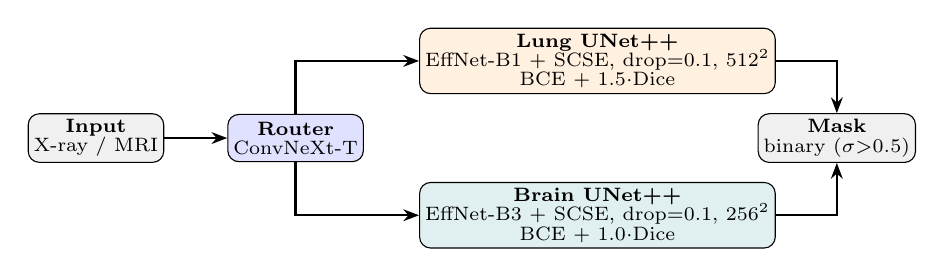
\begin{tikzpicture}[
    node distance=0.55cm and 0.8cm,
    every node/.style={font=\scriptsize},
    box/.style={draw, rounded corners, minimum height=0.6cm, minimum width=1.6cm, align=center, fill=#1!12, inner sep=2pt},
    arr/.style={-{Stealth[length=2mm]}, thick}
]
\node[box=gray] (inp) {\textbf{Input}\\[-1pt]X-ray / MRI};
\node[box=blue, right=of inp] (rtr) {\textbf{Router}\\[-1pt]ConvNeXt-T};
\node[box=orange, above right=0.25cm and 0.7cm of rtr] (sL)
  {\textbf{Lung UNet++}\\[-1pt]EffNet-B1 + SCSE, drop=0.1, 512$^2$\\[-1pt]BCE + 1.5$\cdot$Dice};
\node[box=teal, below right=0.25cm and 0.7cm of rtr] (sB)
  {\textbf{Brain UNet++}\\[-1pt]EffNet-B3 + SCSE, drop=0.1, 256$^2$\\[-1pt]BCE + 1.0$\cdot$Dice};
\node[box=gray, right=5cm of rtr] (out) {\textbf{Mask}\\[-1pt]binary ($\sigma{>}0.5$)};

\draw[arr] (inp) -- (rtr);
\draw[arr] (rtr) |- (sL);
\draw[arr] (rtr) |- (sB);
\draw[arr] (sL) -| (out);
\draw[arr] (sB) -| (out);
\end{tikzpicture}%
}
\caption{Anatomy-aware routing architecture. A ConvNeXt-Tiny classifier routes each input to a dedicated UNet++ specialist with SCSE attention and encoder. The mixed model $S^H$ shares lung backbone (UNet++/EffNet-B1, 256$^2$, BCE + 1.0$\cdot$Dice) but no attention and is trained jointly on both organs.}
\label{fig:routing}
\end{figure}

Since Dice collapse is not observable at deployment time (ground-truth masks are unavailable), we design three complementary post-hoc detection mechanisms that flag unreliable predictions using only model outputs and require no retraining.

\subsection{Uncertainty Estimation}

We employ MC Dropout~\cite{b6,b8,b9} with $T{=}5$ stochastic forward passes per image at inference. For each pixel $(i,j)$, we compute the variance across passes and aggregate into a foreground-weighted scalar:
\begin{equation}
u = \frac{\sum_{ij} \text{Var}_t[\hat{y}_{t,ij}] \cdot \mathbf{1}[\bar{y}_{ij} > 0.05]}{\max(1,\; \sum_{ij} \mathbf{1}[\bar{y}_{ij} > 0.05])}
\label{eq:uncertainty}
\end{equation}
where $\bar{y}_{ij}$ is the mean predicted probability. Restricting to foreground pixels prevents large backgrounds from diluting the signal. We establish a base threshold $u_{\text{thresh}}$ at the 95th percentile of uncertainty values over clean training data. All percentile thresholds in this work are hyperparameters selected empirically for our architecture and calibration set.

\subsection{Domain-Shift Detection}

While MC Dropout captures epistemic uncertainty, it does not directly measure whether the input lies within the model's training distribution. We detect anatomical mismatch via Mahalanobis distance~\cite{b7,b10} in encoder feature space. For each input, we extract the deepest encoder feature map, apply global average pooling and $L_2$ normalisation to obtain a feature vector $\mathbf{z}$, and compute:
\begin{equation}
d_M(\mathbf{z}) = \sqrt{(\mathbf{z} - \boldsymbol{\mu})^\top \hat{\boldsymbol{\Sigma}}^{-1} (\mathbf{z} - \boldsymbol{\mu})}
\label{eq:mahal}
\end{equation}
where $\boldsymbol{\mu}$ is the centroid of pooled (clean+noisy) training features and $\hat{\boldsymbol{\Sigma}}$ is a shrinkage-regularised covariance matrix ($\alpha{=}0.1$, Ledoit--Wolf~\cite{b11}). Unlike cosine distance, Mahalanobis distance accounts for the covariance structure: deviations along low-variance (discriminative) directions are penalised more heavily, giving better separation between in-distribution and out-of-distribution inputs. We establish a base threshold $d_{\text{thresh}}$ at the 87th percentile over calibration data.

\subsection{Plausibility Checks and Composite Flagging}

We apply morphological heuristics to the predicted mask to detect anatomically implausible outputs. A mask is considered \emph{too fragmented} if its number of connected components exceeds the organ-specific maximum ($>2$ components, indicating scattered spurious activations rather than a coherent lesion). A mask is considered \emph{too small} if its area ratio (predicted foreground pixels divided by total image pixels) falls below the organ-specific minimum ($<0.001$, indicating a near-empty prediction where the model effectively abstained).

An image is flagged as unreliable if \emph{any} of four conditions are met: (1) \emph{extreme uncertainty} ($u > 1.3 \cdot u_{\text{thresh}}$); (2) \emph{extreme domain shift} ($d_m > 1.3 \cdot d_{\text{thresh}}$); (3) a \emph{combinatorial flag} where both signals are moderately elevated ($u > 0.6 \cdot u_{\text{thresh}}$ and $d_m > 1.0 \cdot d_{\text{thresh}}$); or (4) a \emph{geometric flag} where structural anomalies co-occur with domain shift. Specifically, the geometric flag is raised if the mask is too fragmented and $d_m > 1.2 \cdot d_{\text{thresh}}$, or if it is too small and $d_m > 1.25 \cdot d_{\text{thresh}}$. Requiring this co-occurrence prevents morphological heuristics from unnecessarily firing on structurally unusual but in-distribution masks.

A potential fourth basic signal, re-querying the router for its classification confidence on the input, was intentionally excluded. As the router is near-perfect, this signal alone would flag virtually all misrouted cases and prevent flagging correctly routed cases with near-perfect reliability, suppressing the contribution of the other three mechanisms and the combined framework itself. We omit it here to provide a conservative evaluation of the post-hoc detection channels themselves. In a practical deployment, router-confidence verification would serve as an additional safety layer.

%==============================================================
\section{Experiments and Results}
%==============================================================

\subsection{Experimental Setup}

Lung segmentation uses a community-repackaged PNG version of the SIIM-ACR Pneumothorax competition data~\cite{b12,b13} (12,047 X-rays, binary masks). Brain segmentation uses LGG FLAIR MRI dataset~\cite{b14} (3,929 slices, 110 patients). Both are split 70/15/15\% train/val/test with stratified sampling.

All models use UNet++ with EfficientNet encoders and BCE\,+\,Dice loss. Specialists employ SCSE attention~\cite{b15} and 0.1 decoder dropout. The mixed model omits attention because organ-specific spatial priors (e.g., ``focus on lung periphery'' vs.\ ``focus on cortical regions'') conflict when learned jointly, making shared attention counterproductive. Training uses AdamW~\cite{b16} with cosine-annealing scheduling and mixed-precision (FP16). Augmentations (flips, mild rotations, brightness/contrast) are tailored per-organ: brain omits horizontal flip due to anatomical laterality, while lung uses conservative geometric parameters to preserve thin pneumothorax structures. Gaussian noise ($\sigma \in [0.08, 0.12]$) is added in normalised pixel space at test time to simulate mild acquisition perturbation, applied identically across all models. Individual-model training additionally applies class weight rebalancing, validation-set threshold optimisation, and optional test-time augmentation.

\subsection{Evaluation Scenarios}

We evaluate six scenarios per organ domain (Table~\ref{tab:scenarios}). Cases~1--4 represent operational conditions; Cases~5--6 simulate misrouting under noisy and clean inputs, respectively. Although our router achieves near-perfect accuracy in the binary lung-vs-brain setting, we include clean misrouting (Case~6) to study failure detectability under conditions directly relevant to finer-grained routing tasks (e.g., routing among disease-specific specialists within the same organ), where classifier confusion is more likely even on clean inputs.

\begin{table}[t]
\centering
\caption{Evaluation scenarios per organ domain.}
\label{tab:scenarios}
\vspace{-4pt}
\renewcommand{\arraystretch}{1.05}
\begin{tabular}{@{}clcc@{}}
\toprule
\textbf{Case} & \textbf{System} & \textbf{Routing} & \textbf{Input} \\
\midrule
1 & $S^O$ (specialist) & Correct & Clean \\
2 & $S^H$ (mixed) & --- & Clean \\
3 & $S^O$ (specialist) & Correct & Noisy \\
4 & $S^H$ (mixed) & --- & Noisy \\
5 & $S^O$ (specialist) & Forced wrong & Noisy \\
6 & $S^O$ (specialist) & Forced wrong & Clean \\
\bottomrule
\end{tabular}
\vspace{-6pt}
\end{table}

\subsection{Segmentation Results}

Table~\ref{tab:combined} reports both segmentation performance and composite-detector flag rates across all routing scenarios ($n{=}1000$ per domain, stratified).

Three patterns are visible across both domains. First, specialisation improves both accuracy and robustness under correct routing: the anatomy-aware system consistently outperforms the mixed model by +8.59 (brain) and +14.35 (lung) Dice on clean data. Second, misrouting causes sharp Dice collapse by 38--78 points when the wrong specialist is applied, regardless of input quality (Fig.~\ref{fig:boxplots}). Third, the mixed model degrades gradually but without any alarm; its decline produces no signal easily distinguishable from normal operation. This asymmetry between sharp-detectable and gradual-silent failure motivates the detectability analysis below.

\begin{figure}[t]
\centering
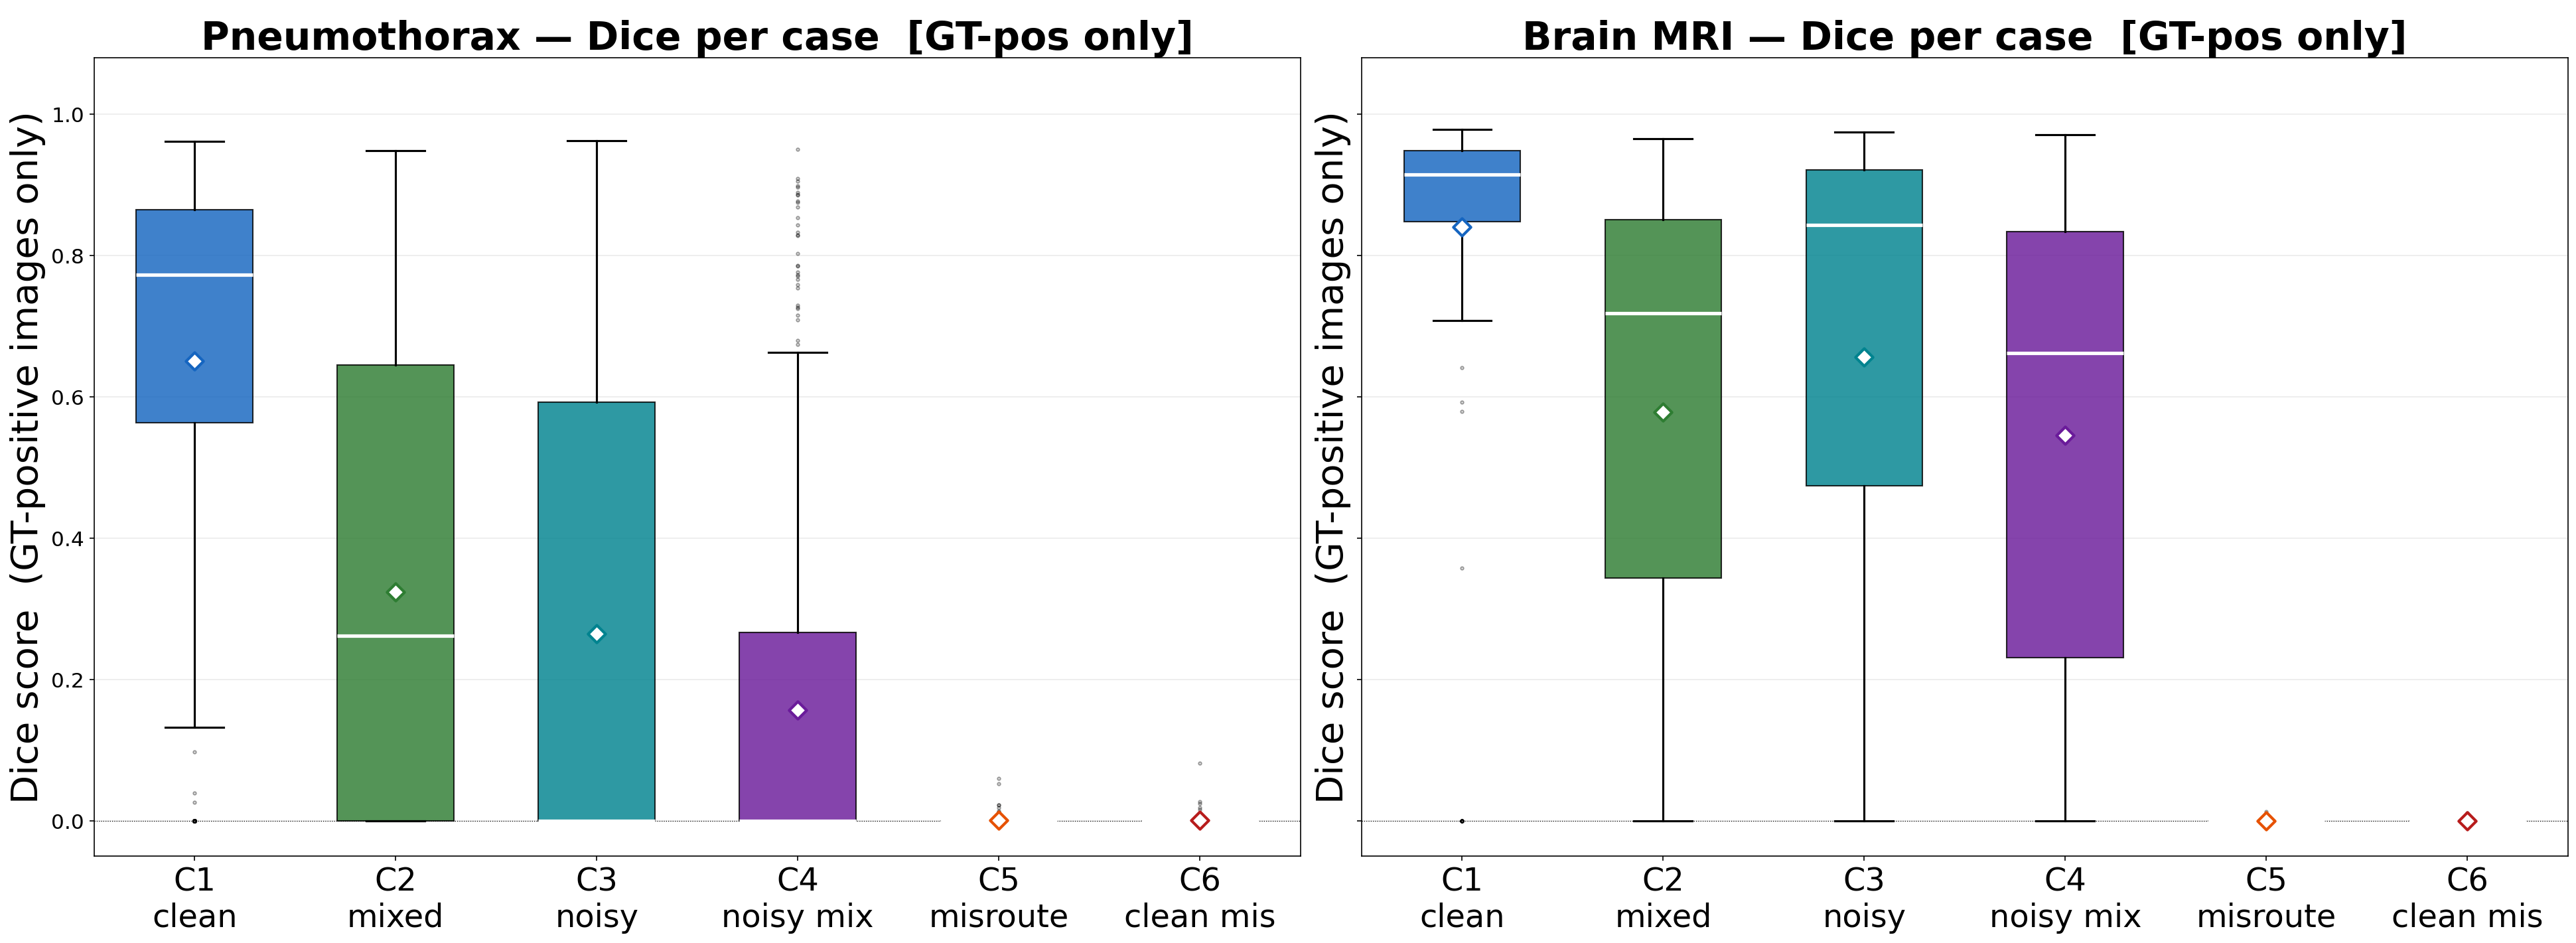
\includegraphics[width=0.95\columnwidth]{viz4_dice_boxplots.png}
\caption{Per-case Dice distributions. Specialists under correct routing (C1, C3) are tight and high; misrouting (C5, C6) collapses the median; the mixed model (C2, C4) lies between.}
\label{fig:boxplots}
\end{figure}

\subsection{Failure Detectability}

Beyond segmentation accuracy, Table~\ref{tab:combined} reports per-signal and composite flag rates for all cases. The key finding is the asymmetry in detectability.

\begin{table*}[t]
\centering
\caption{Segmentation and failure-detection results. $\bar{d}_M$ = mean Mahalanobis distance. Geom = morphological plausibility flag rate. Combo = combinatorial (unc+shift) flag rate. Flag = composite flag rate across all four conditions (extreme uncertainty, extreme shift, combinatorial, geometric). FP\textsubscript{raw}/FP\textsubscript{sys} = model/system-level false-positive rate. Sys Dice = system-level Dice (flagged images contribute 0).}
\label{tab:combined}
\vspace{-4pt}
\renewcommand{\arraystretch}{0.85}
\setlength{\tabcolsep}{5.5pt}
{\scriptsize
\begin{tabular}{@{}llcccccccccc@{}}
\toprule
& \textbf{Case} & \textbf{Dice} & \textbf{IoU} & \textbf{$\bar{u}$} & \textbf{$\bar{d}_M$} & \textbf{Geom} & \textbf{Combo} & \textbf{Flag} & \textbf{FP\textsubscript{raw}} & \textbf{FP\textsubscript{sys}} & \textbf{Sys Dice} \\
\midrule
\multirow{6}{*}{\rotatebox{90}{\scriptsize Pneumo}}
& C1 $S^O$ clean      & \textbf{.839} & \textbf{.796} & .023 & 14.22 & .027 & .052 & .115 & .037 & .012 & .802 \\
& C2 $S^H$ clean      & .695 & .664 & .023 & 17.65 & .051 & .084 & .172 & .058 & .022 & .657 \\
& C3 $S^O$ noisy      & .684 & .659 & .033 & 11.01 & .038 & .049 & .108 & .038 & .013 & .659 \\
& C4 $S^H$ noisy      & .639 & .623 & .020 & 17.62 & .048 & .097 & .173 & .040 & .008 & .613 \\
& C5 $S^O$ misrt.\ noisy & .058 & .058 & .055 & 31.39 & .247 & .425 & \textbf{1.000} & .903 & .000 & .058 \\
& C6 $S^O$ misrt.\ clean & .153 & .153 & .033 & 31.90 & .252 & .323 & \textbf{1.000} & .745 & .000 & .153 \\
\midrule
\multirow{6}{*}{\rotatebox{90}{\scriptsize Brain}}
& C1 $S^O$ clean      & \textbf{.933} & \textbf{.907} & .005 & 20.35 & .015 & .039 & .090 & .018 & .003 & .907 \\
& C2 $S^H$ clean      & .847 & .812 & .017 & 18.08 & .051 & .081 & .183 & .010 & .003 & .794 \\
& C3 $S^O$ noisy      & .874 & .847 & .010 & 18.37 & .019 & .044 & .103 & .010 & .000 & .838 \\
& C4 $S^H$ noisy      & .829 & .795 & .019 & 17.72 & .056 & .080 & .156 & .021 & .010 & .777 \\
& C5 $S^O$ misrt.\ noisy & .556 & .556 & .055 & 21.22 & .100 & .331 & .707 & .148 & .016 & .556 \\
& C6 $S^O$ misrt.\ clean & .510 & .510 & .061 & 23.35 & .217 & .378 & \textbf{.963} & .218 & .003 & .510 \\
\bottomrule
\end{tabular}
}
\vspace{-8pt}
\end{table*}

The composite detector exhibits a clear asymmetry. Misrouted cases (5--6) are flagged at near-total rates by the extreme and combinatorial logic conditions, while the mixed model under noise (Case~4) is flagged only marginally, leaving its gradual decline largely invisible to the monitoring system unless thresholds are tuned aggressively. The system-level false-positive rate (FP\textsubscript{sys}) demonstrates the safety value of abstention: model-level FP rates as high as 90.3\% on misrouted pneumothorax are reduced to 0.0\% after flagging. Fig.~\ref{fig:uncmaps} shows representative predictions with pixel-level uncertainty overlays: correctly routed cases exhibit low, uniform uncertainty, while misrouted cases produce high uncertainty concentrated around spurious activations. The per-signal flag decomposition is shown in Fig.~\ref{fig:flag_breakdown}.

\begin{figure}[t]
\centering
\begin{subfigure}[t]{0.46\columnwidth}
    \centering
    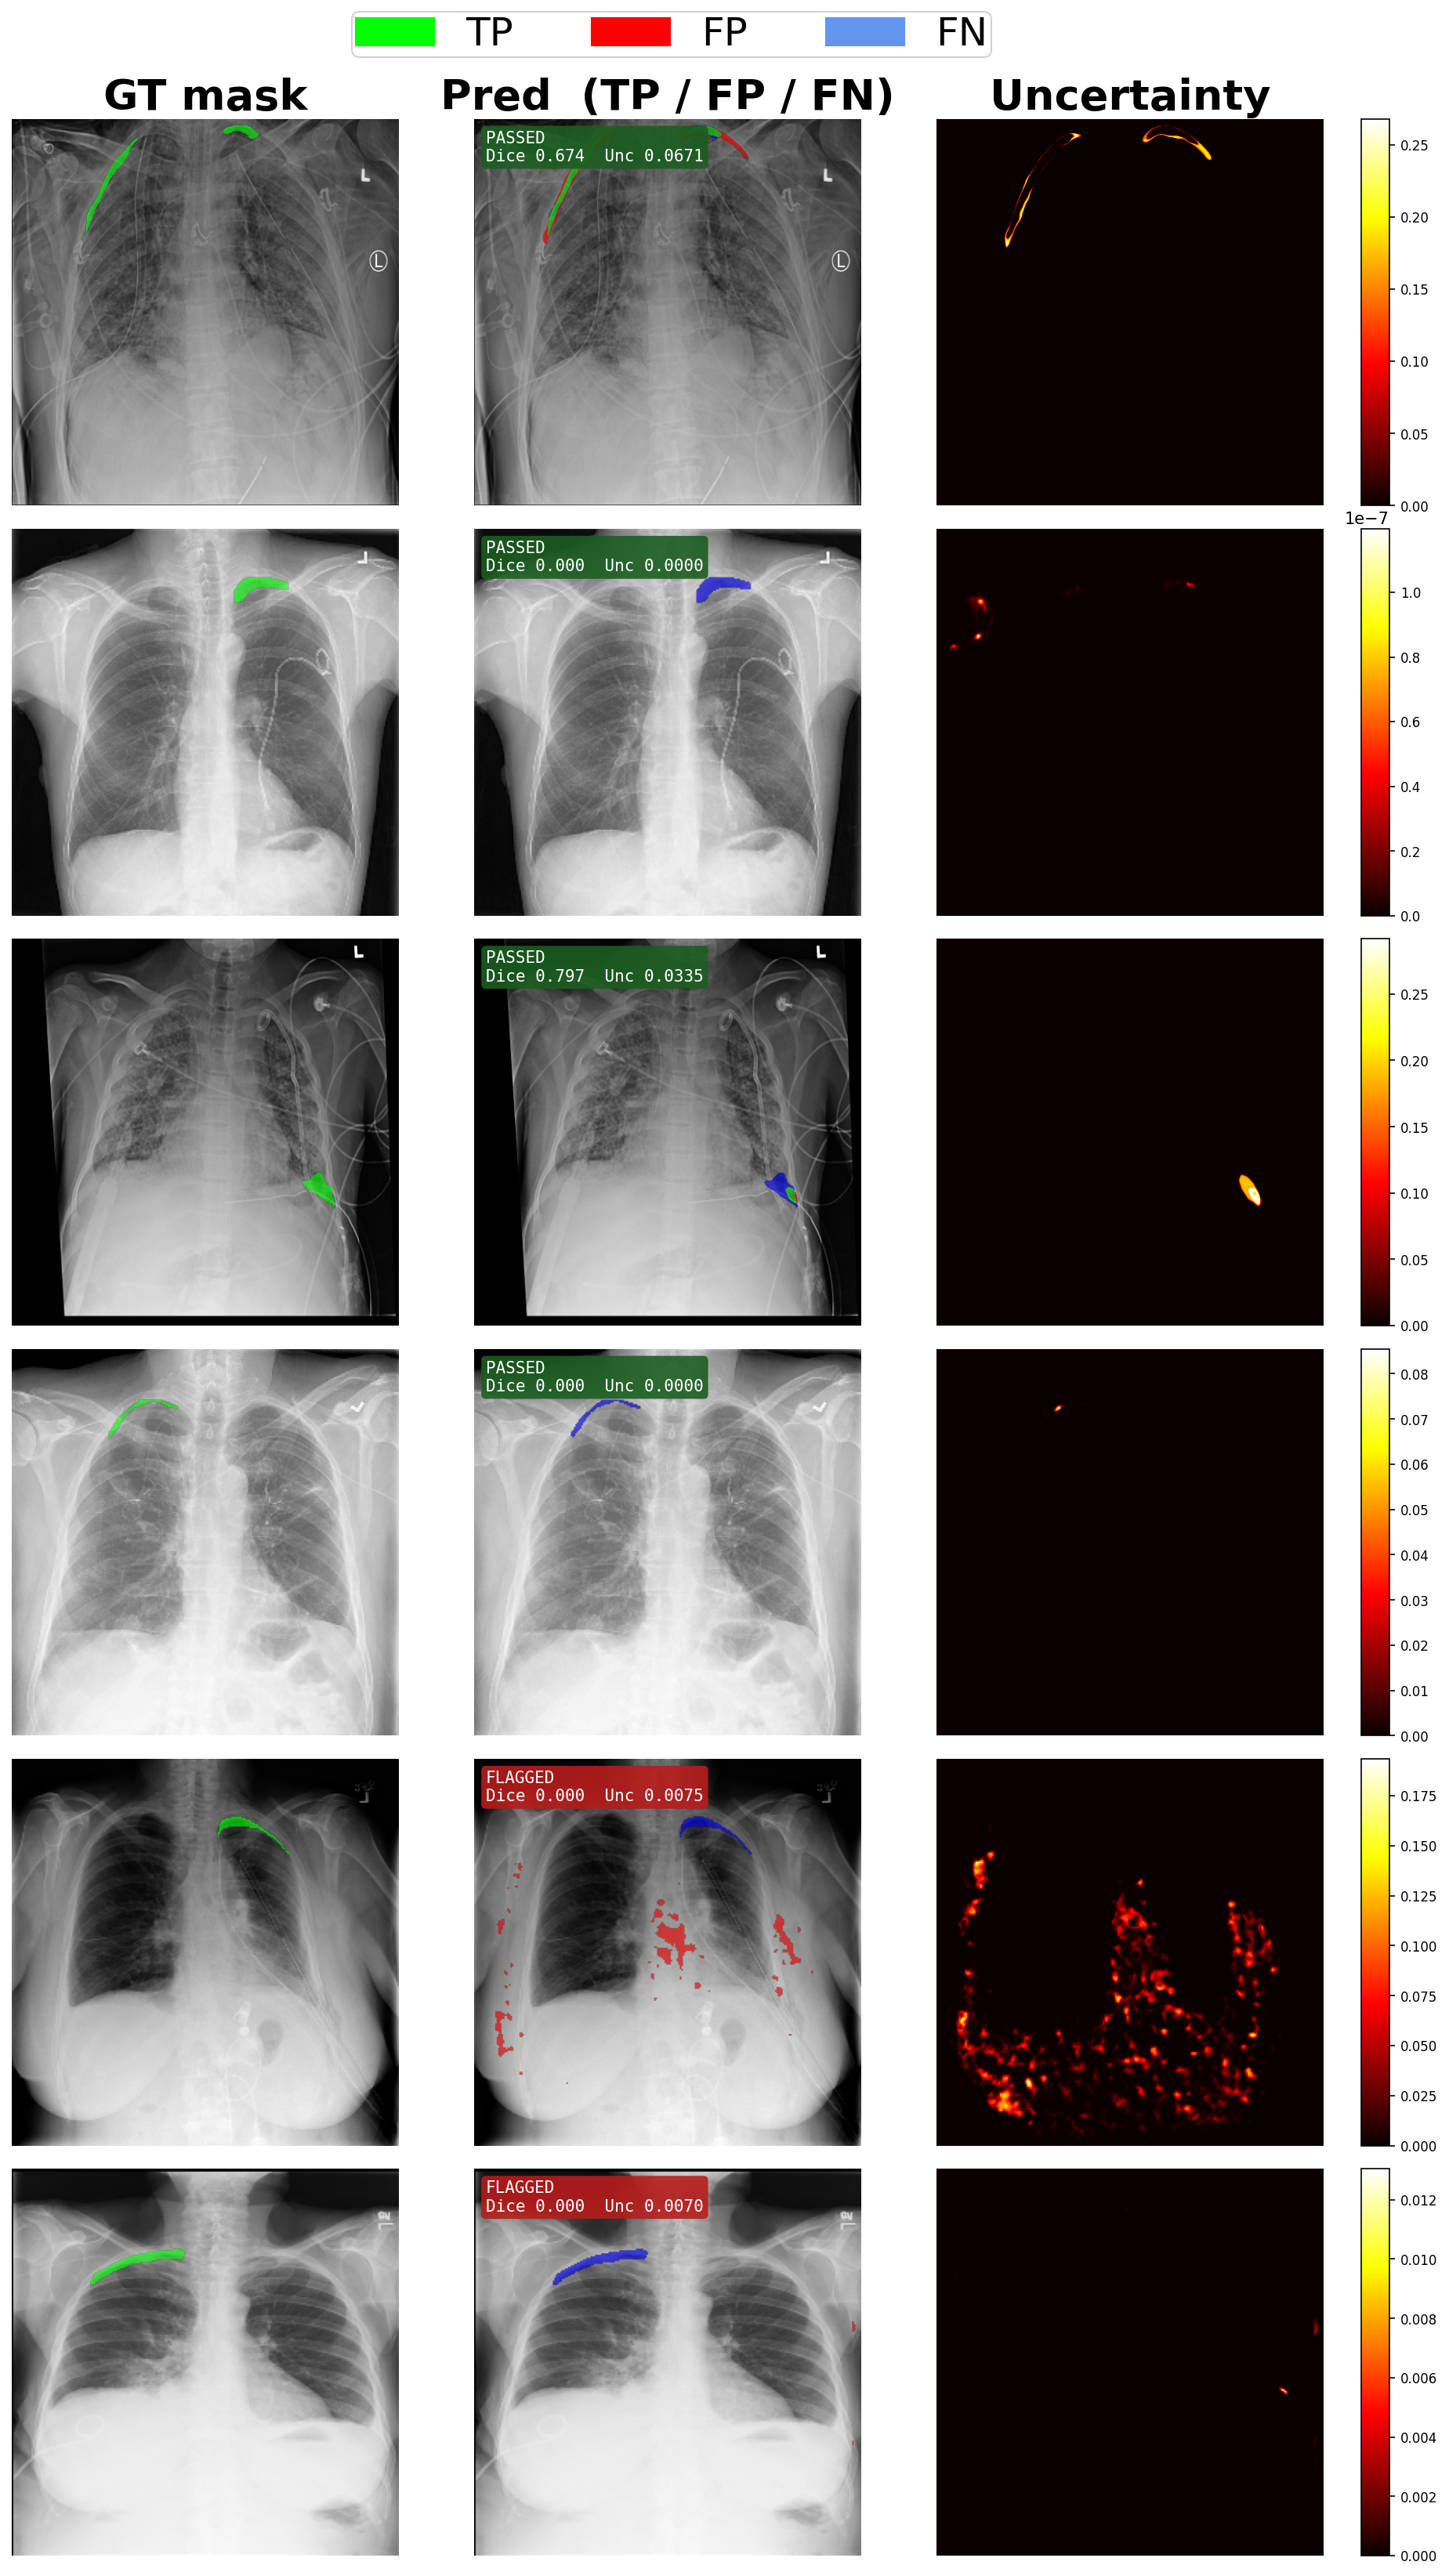
\includegraphics[width=\linewidth]{viz2_uncertainty_maps.png}
    \caption{Pneumothorax specialist}
    \label{fig:viz2a}
\end{subfigure}
\hfill
\begin{subfigure}[t]{0.46\columnwidth}
    \centering
    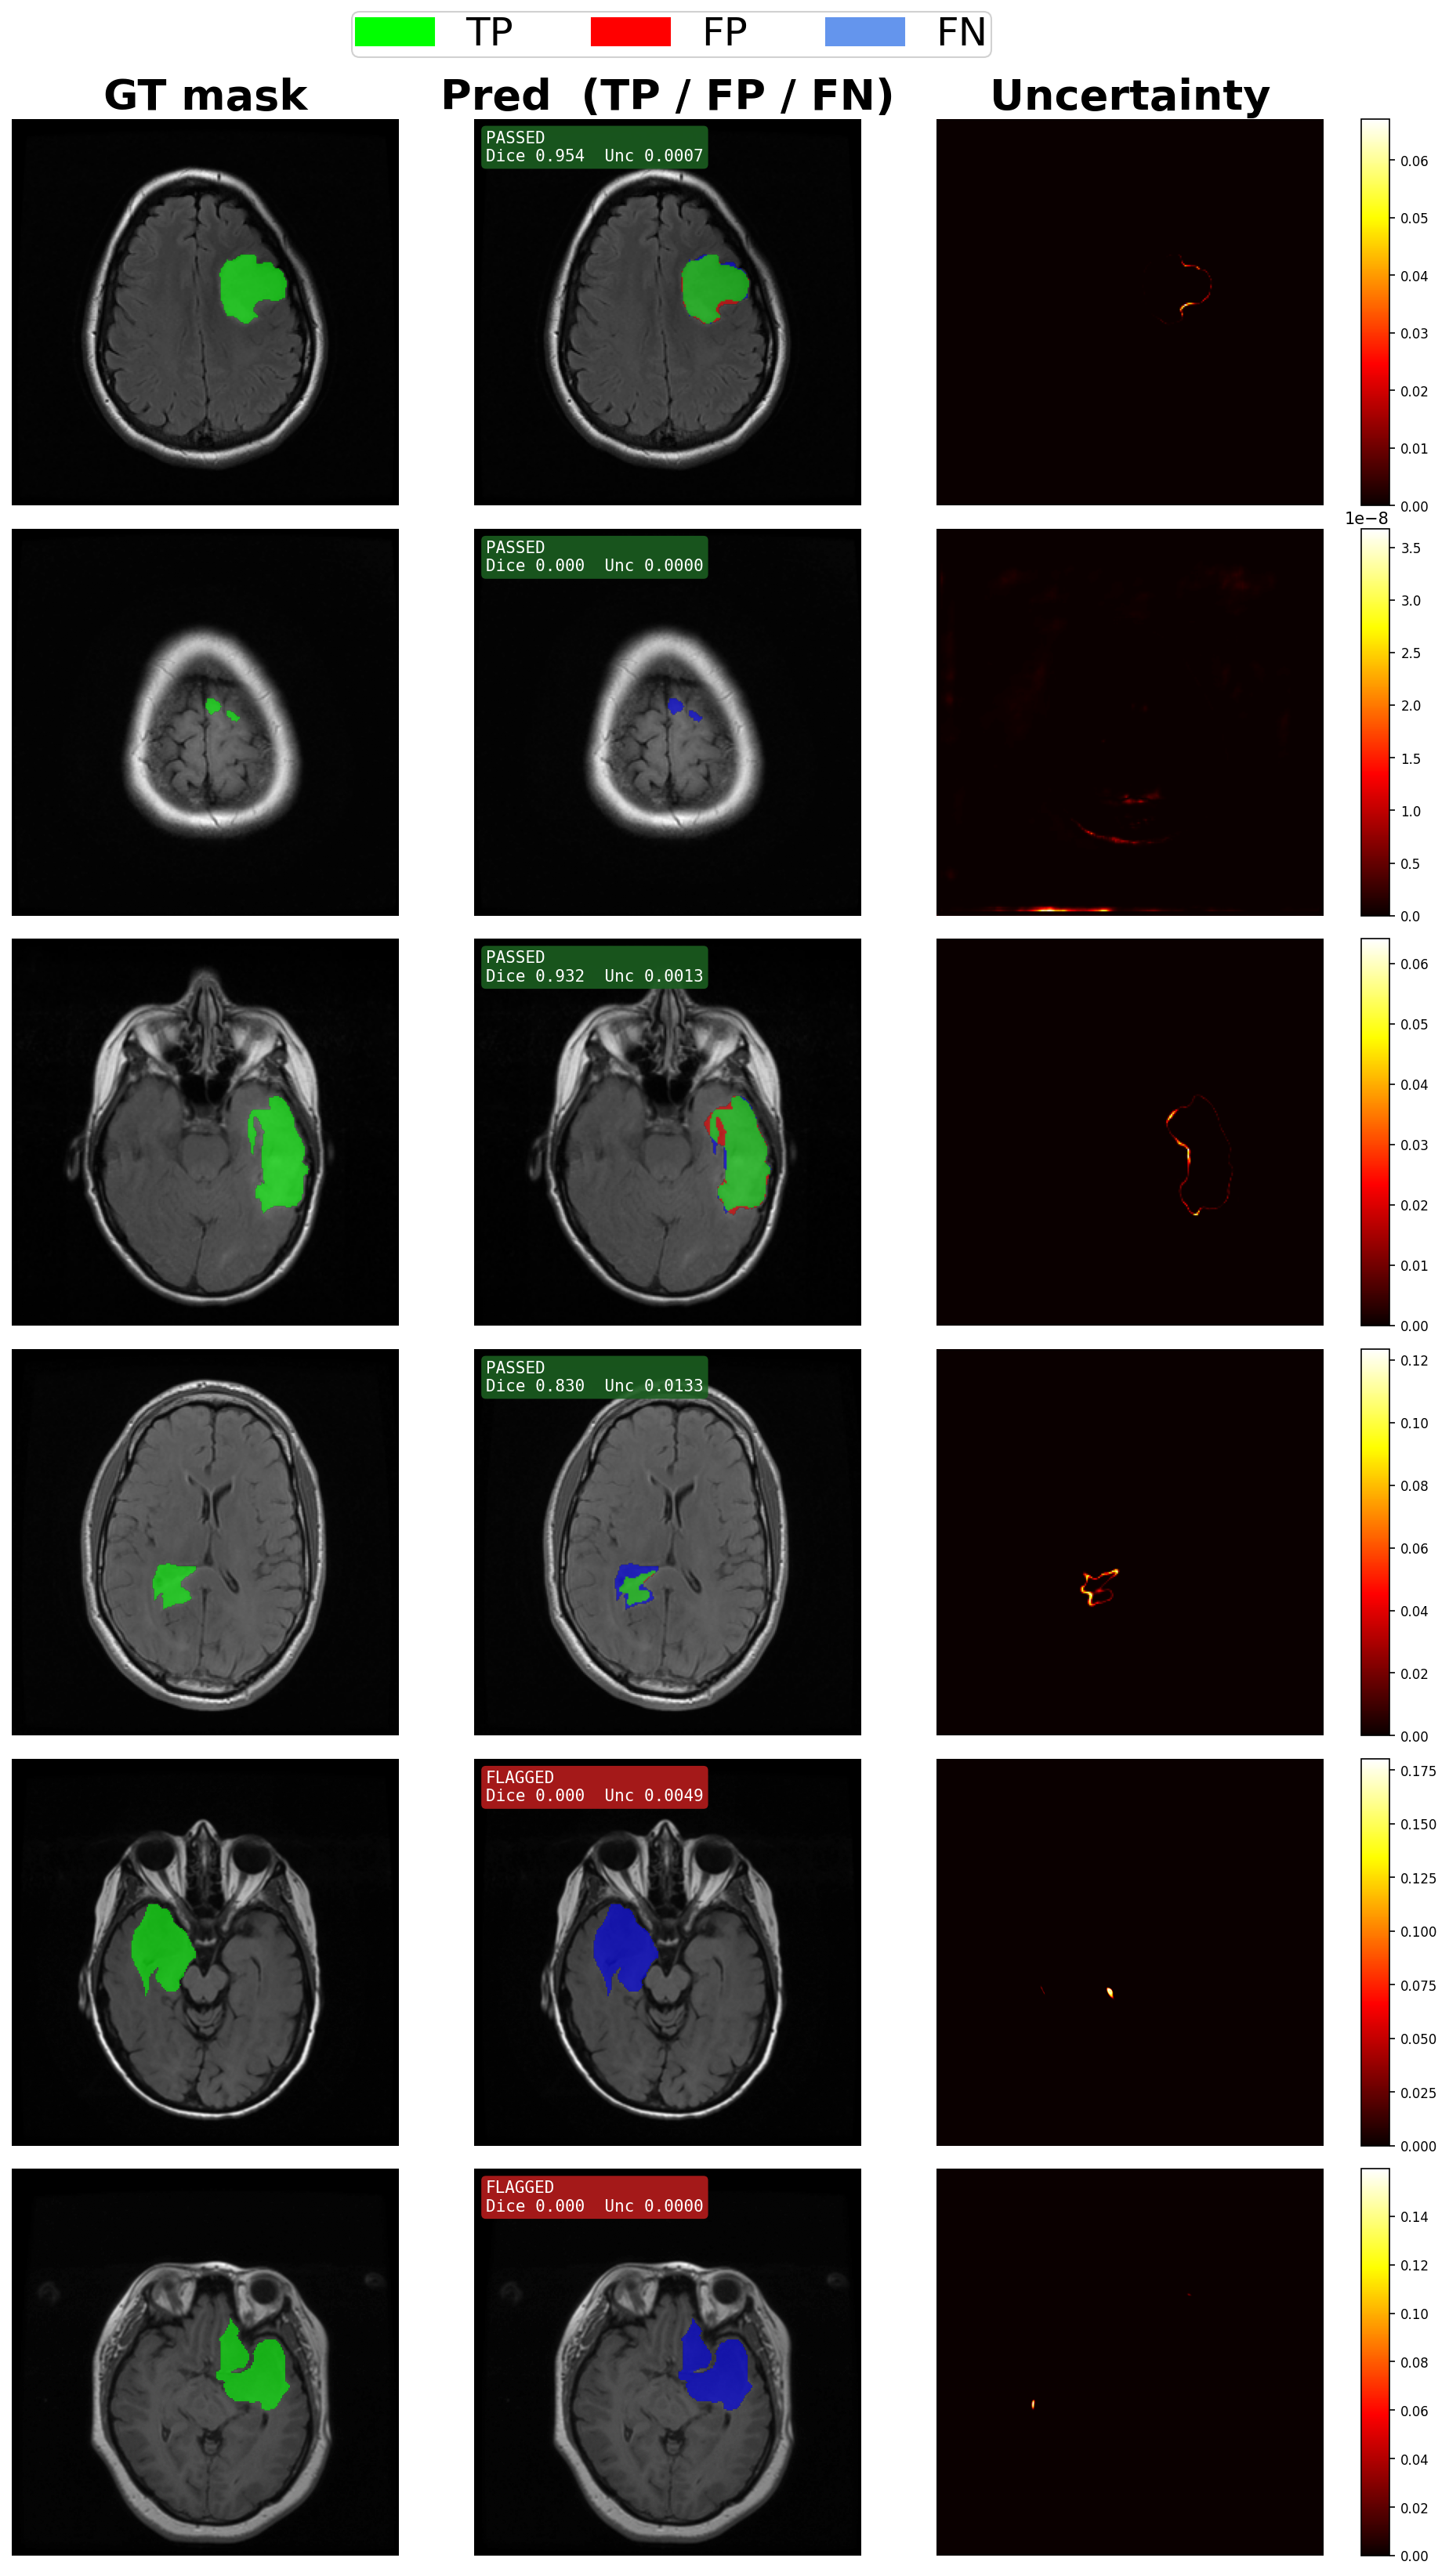
\includegraphics[width=\linewidth]{viz2b_uncertainty_maps.png}
    \caption{Brain MRI specialist}
    \label{fig:viz2b}
\end{subfigure}
\caption{MC-Dropout uncertainty overlays. Low uncertainty (dark) marks confident routing; high uncertainty (bright) marks misrouting/noise.}
\label{fig:uncmaps}
\end{figure}

\begin{figure}[t]
\centering
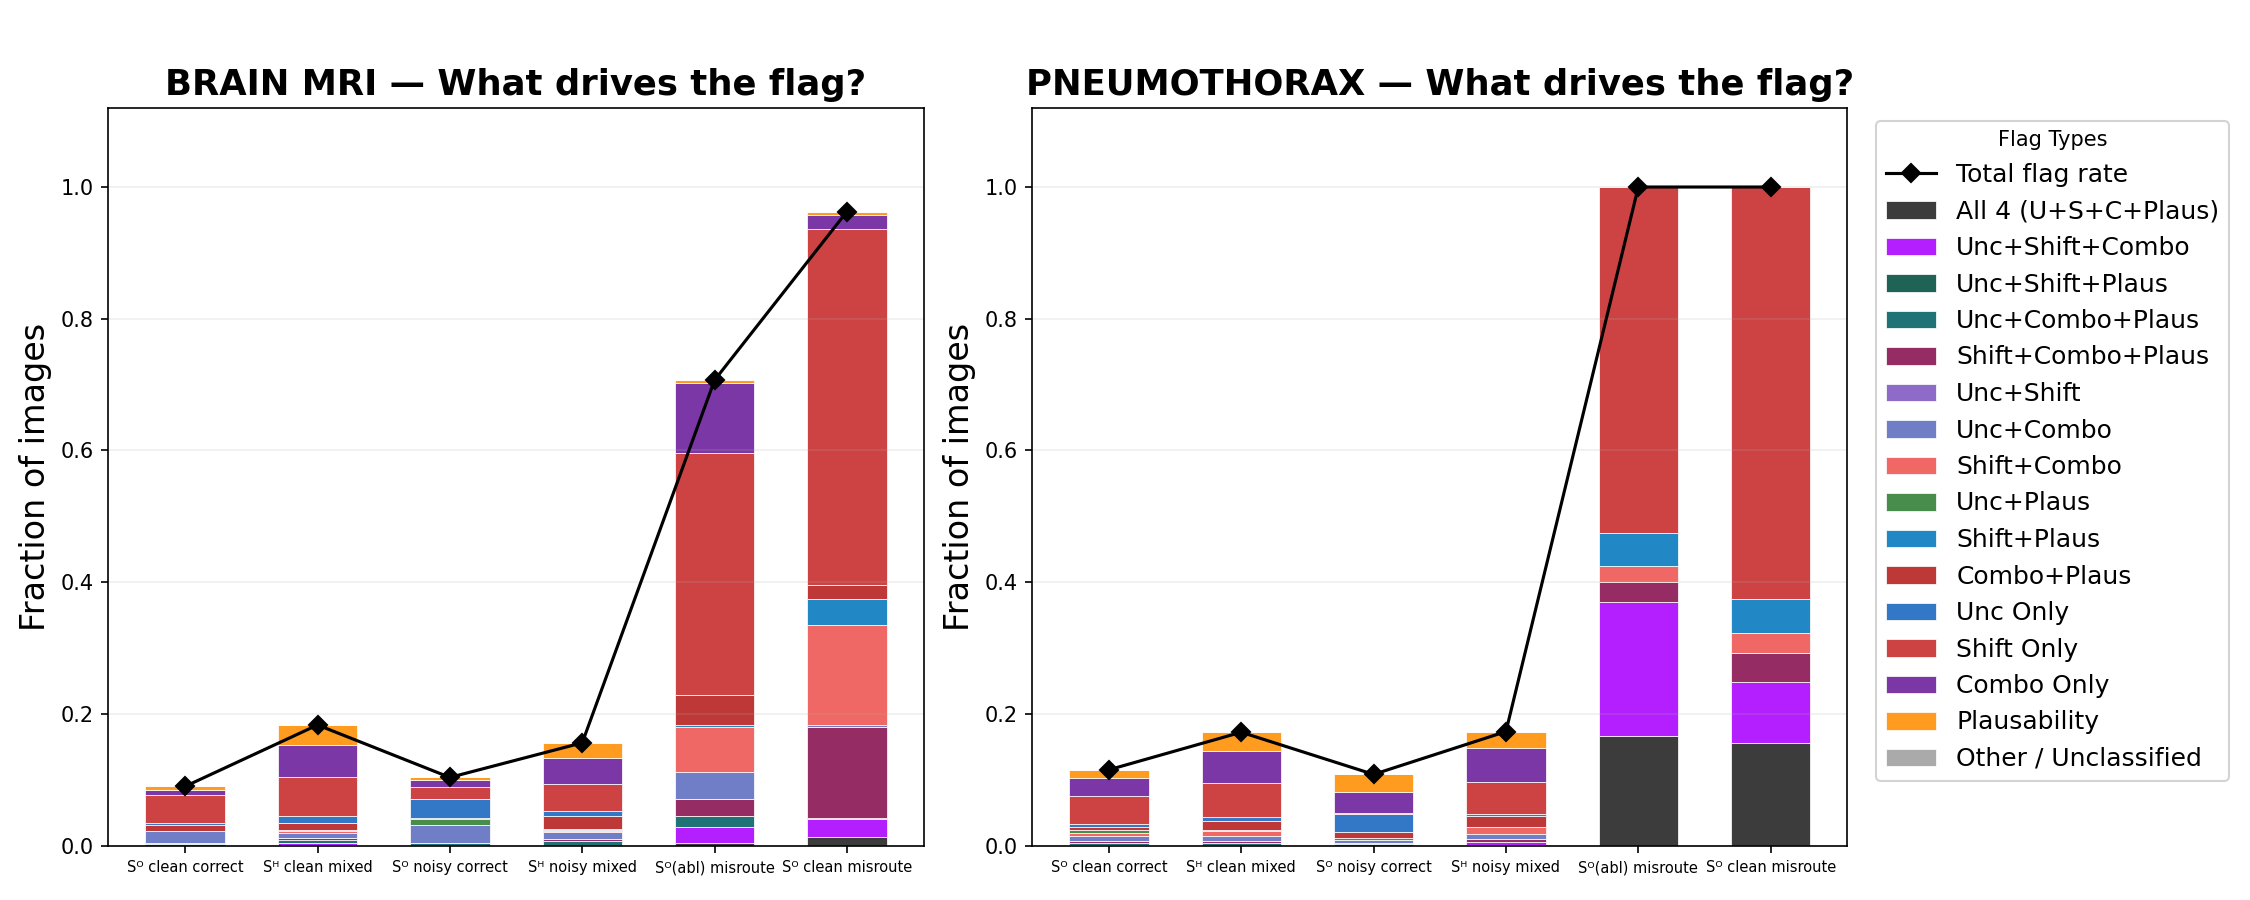
\includegraphics[width=0.95\columnwidth]{viz5_flag_breakdown.png}
\caption{Flag decomposition per case. Domain-shift (orange) dominates misroutes; uncertainty (blue) is complementary.}
\label{fig:flag_breakdown}
\end{figure}

\begin{figure}[t]
\centering
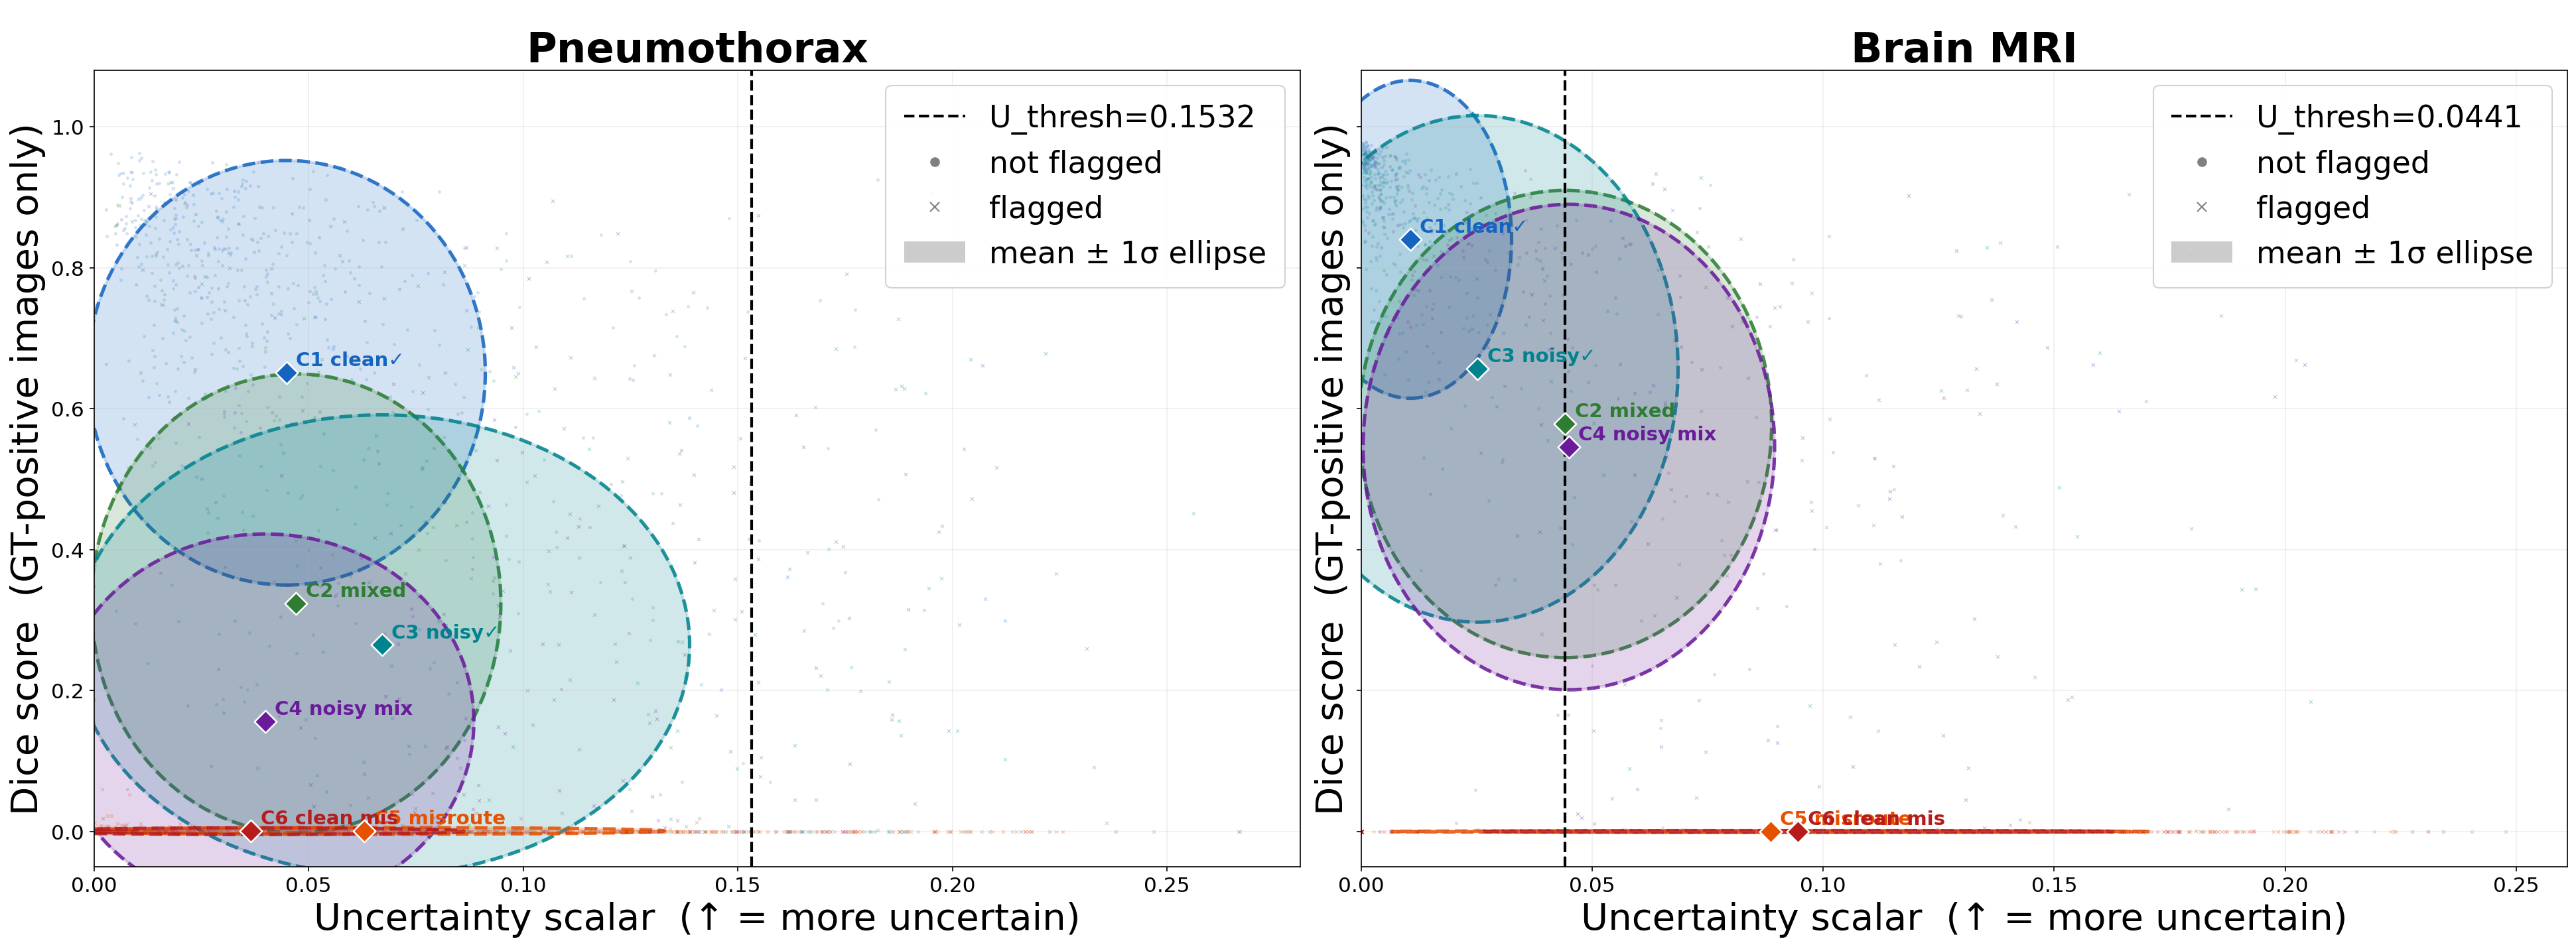
\includegraphics[width=0.95\columnwidth]{viz1_uncertainty_vs_dice.png}
\caption{Uncertainty vs.\ Dice per image. Correct routing (C1--C4) clusters low-unc/high-Dice; misroutes (C5, C6) shift high-unc/low-Dice.}
\label{fig:scatter}
\end{figure}

Misrouting produces anomalous signals across all detection channels: elevated uncertainty, large domain-shift distances, and morphological implausibility. Fig.~\ref{fig:scatter} confirms that uncertainty correlates strongly with Dice degradation at per-image level, supporting its use as a failure indicator. This composite detection is entirely absent in mixed models. The anatomy-aware system \emph{fails loudly}; the mixed model fails silently.

%==============================================================
\section{Conclusion}
%==============================================================

We demonstrated that anatomy-aware routing with specialist UNet++ models improves segmentation accuracy by +8.6 (brain) and +14.4 (lung) Dice points over a mixed-domain baseline under both clean and noisy conditions. A composite post-hoc detector exploiting MC-Dropout uncertainty, Mahalanobis domain-shift scores, and mask morphology flagged 70.7--100\% of degraded predictions across all test cases, with great room for improvement using router confidence flagging. By contrast, mixed models degraded silently under the same conditions, with flag rates of at most 17.3\%.

These results point to a clear design trade-off. The mixed model never collapses catastrophically (worst-case Dice of 0.639 remains within operational range), but its errors are indistinguishable from normal variance. The anatomy-aware system achieves higher peak accuracy, yet misrouting produces sharp collapse. This collapse, however, is accompanied by anomalous reliability signals across all three detection channels, which makes it automatically detectable. In safety-critical settings, a failure that triggers an alarm and can be caught is preferable to one that goes unnoticed.

The anatomy-aware system also provides layered safety: (i)~high-confidence routing makes misrouting rare; (ii)~the composite failure detector catches it when it occurs; (iii)~flagged predictions trigger fallback, whether deferral to mixed models, human review, or explicit abstention. The framework reduces false-positives from 90.3\% to 0.0\% on misrouted pneumothorax cases, confirming that anatomy-aware pipelines combine higher accuracy with the ability to \emph{fail loudly} and support safer clinical deployment.

Our two-organ scope reflects compute constraints (single Tesla P100 with limited free-tier runtime); scaling to $k>2$ specialists remains untested. The synthetic Gaussian noise model may not capture realistic acquisition artefacts (motion blur, metal artefacts, scanner drift), and the empirically chosen detection thresholds would need recalibration for new hardware or populations. Future work will extend the framework to multi-organ routing, investigate learned plausibility checks, incorporate explainability techniques such as Grad-CAM, and validate on clinical data with real-world distribution shifts.

%==============================================================
% REFERENCES
%==============================================================
\begin{thebibliography}{00}
\bibitem{b1} O.~Ronneberger, P.~Fischer, and T.~Brox, ``U-Net: convolutional networks for biomedical image segmentation,'' in \emph{Proc.\ MICCAI}, 2015, pp.~234--241.
\bibitem{b2} Z.~Zhou, M.~M.~R.~Siddiquee, N.~Tajbakhsh, and J.~Liang, ``UNet++: a nested U-Net architecture for medical image segmentation,'' in \emph{Proc.\ DLMIA/ML-CDS}, 2018, pp.~3--11.
\bibitem{b3} Z.~Hong \emph{et al.}, ``Out-of-distribution detection in medical image analysis: a survey,'' \emph{arXiv:2404.18279}, 2024.
\bibitem{b4} D.~Hendrycks and T.~Dietterich, ``Benchmarking neural network robustness to common corruptions and perturbations,'' in \emph{Proc.\ ICLR}, 2019.
\bibitem{b5} A.~Jungo \emph{et al.}, ``On the effect of inter-observer variability for a reliable estimation of uncertainty of medical image segmentation,'' in \emph{Proc.\ MICCAI}, 2018, pp.~682--690.
\bibitem{b6} Y.~Gal and Z.~Ghahramani, ``Dropout as a Bayesian approximation: representing model uncertainty in deep learning,'' in \emph{Proc.\ ICML}, 2016, pp.~1050--1059.
\bibitem{b7} K.~Lee, K.~Lee, H.~Lee, and J.~Shin, ``A simple unified framework for detecting out-of-distribution samples and adversarial attacks,'' in \emph{Proc.\ NeurIPS}, 2018, pp.~7167--7177.
\bibitem{b8} T.~Nair, D.~Precup, D.~L.~Arnold, and T.~Arbel, ``Exploring uncertainty measures in deep networks for multiple sclerosis lesion detection and segmentation,'' \emph{Med.\ Image Anal.}, vol.~59, 2020, Art.~no.~101557.
\bibitem{b9} S.~Wang \emph{et al.}, ``Towards generalizable medical image segmentation with pixel-wise uncertainty estimation,'' \emph{arXiv:2305.07883}, 2023.
\bibitem{b10} A.~Vasiliuk, D.~Frolova, M.~Belyaev, and B.~Shirokikh, ``Limitations of out-of-distribution detection in 3D medical image segmentation,'' \emph{J.\ Imaging}, vol.~9, no.~9, 2023, Art.~no.~191.
\bibitem{b11} O.~Ledoit and M.~Wolf, ``A well-conditioned estimator for large-dimensional covariance matrices,'' \emph{J.\ Multivariate Anal.}, vol.~88, no.~2, pp.~365--411, 2004.
\bibitem{b12} ``SIIM-ACR Pneumothorax Segmentation,'' Society for Imaging Informatics in Medicine, 2019. [Online]. Available: \url{https://www.kaggle.com/c/siim-acr-pneumothorax-segmentation}
\bibitem{b13} ``Chest X-Ray Images with Pneumothorax Masks,'' Kaggle, 2019. [Online]. Available: \url{https://www.kaggle.com/datasets/vbookshelf/pneumothorax-chest-xray-images-and-masks}
\bibitem{b14} M.~Buda, A.~Saha, and M.~A.~Mazurowski, ``Association of genomic subtypes of lower-grade gliomas with shape features automatically extracted by a deep learning algorithm,'' \emph{Comput.\ Biol.\ Med.}, vol.~109, pp.~218--225, 2019. [Online]. Available: \url{https://www.kaggle.com/datasets/mateuszbuda/lgg-mri-segmentation}
\bibitem{b15} A.~G.~Roy, N.~Navab, and C.~Wachinger, ``Concurrent spatial and channel squeeze \& excitation in fully convolutional networks,'' in \emph{Proc.\ MICCAI}, 2018, pp.~421--429.
\bibitem{b16} D.~P.~Kingma and J.~Ba, ``Adam: a method for stochastic optimization,'' in \emph{Proc.\ ICLR}, 2015.
\end{thebibliography}

\end{document}
